\documentclass[11pt]{article}
\usepackage[hw]{eecs126}
\usepackage{pdfpages}

\begin{document}
\courseheader{Lab 03}

\begin{problems}
    \item \begin{problem}[Q2a: Bringing Particles to Life]

        \begin{center}
        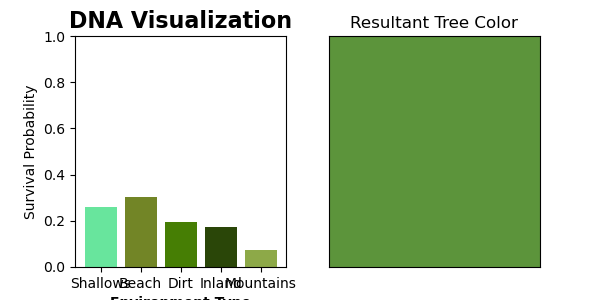
\includegraphics[width=0.5\textwidth]{outputs/q2a_frame0.png}
        
        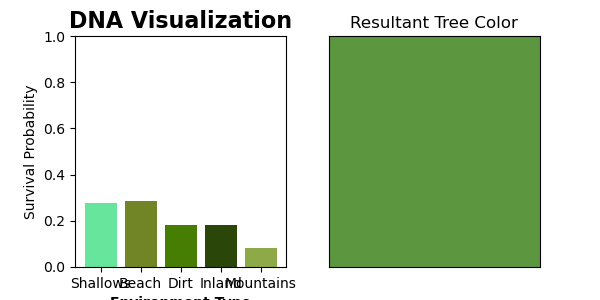
\includegraphics[width=0.5\textwidth]{outputs/q2a_frame15.png}
        
        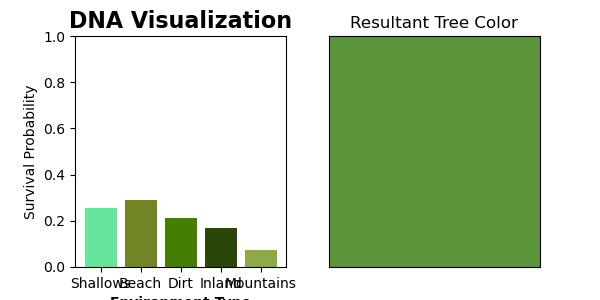
\includegraphics[width=0.5\textwidth]{outputs/q2a_frame29.png}
        \end{center}
    \end{problem}
    \clearpage

    
    \item \begin{problem}[Q3b: Defining the mechanics]

    \begin{enumerate}[(a)]
        \item \textbf{Image outputs}
        \begin{center}
        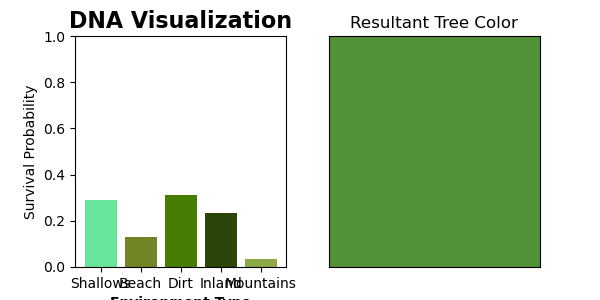
\includegraphics[width=0.5\textwidth]{outputs/q3b_frame0.png}
        
        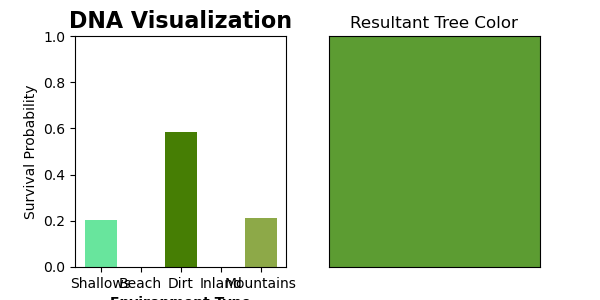
\includegraphics[width=0.5\textwidth]{outputs/q3b_frame25.png}
        
        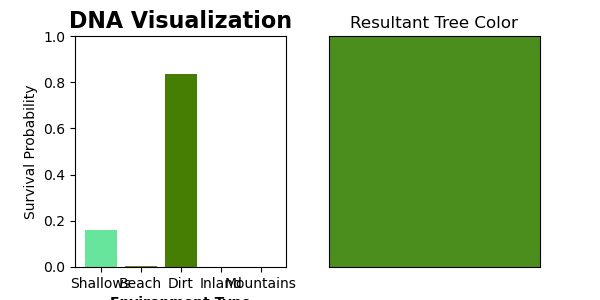
\includegraphics[width=0.5\textwidth]{outputs/q3b_frame49.png}
        \end{center}

        \item \textbf{Text responses}

        Based on your investigations, answer the following questions:

        \begin{enumerate}[(i)]
            \item What would you guess is the environment type of the square?

            \begin{solution}
                
            \end{solution}
            
            \item How does mutation variance affect the rate of convergence and the behavior once evolution has reached steady state?

            \begin{solution}
                
            \end{solution}
            
            \item In a rapidly changing environment, would we want a high or low mutation rate? What about in a predictable environment?

            \begin{solution}
                
            \end{solution}
            
            \item How does the competition constant affect rate of convergence and the behavior once evolution has reached steady state?

            \begin{solution}
                
            \end{solution}
        \end{enumerate}
    \end{enumerate}
        
    \end{problem}
    
    \clearpage
    
    \item \begin{problem}[Q4: Putting it all together]

    \begin{enumerate}[(a)]
        \item \textbf{Image outputs}
        
        \begin{center}
        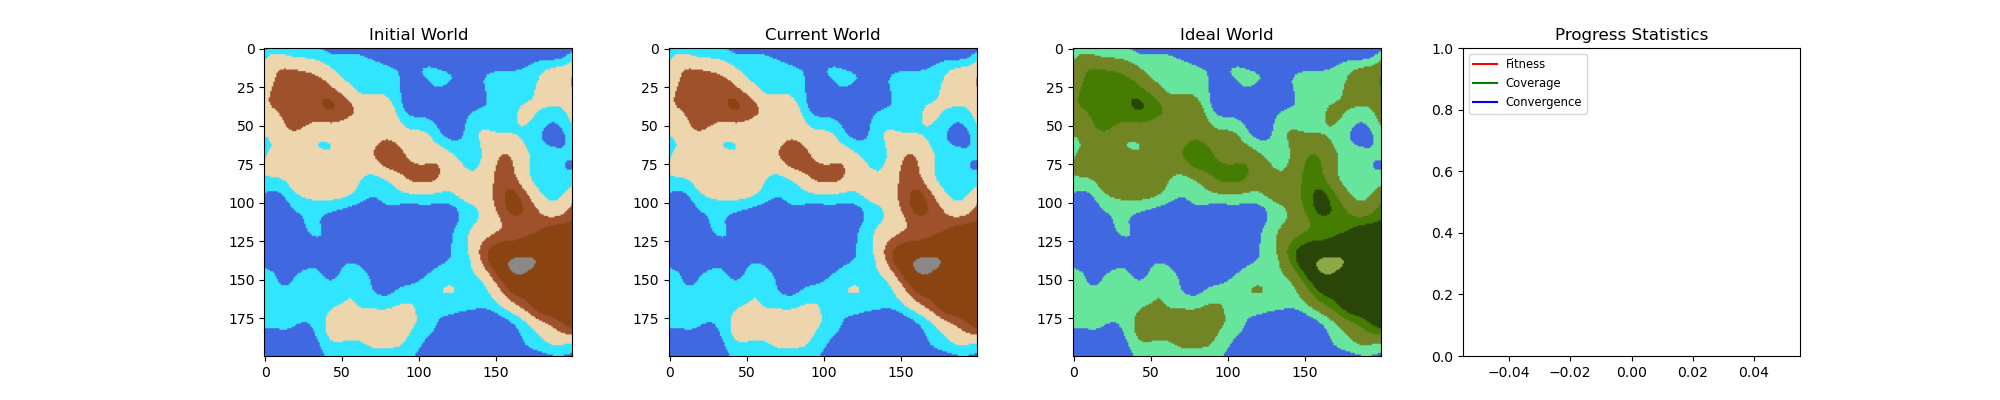
\includegraphics[width=\linewidth]{outputs/q4_frame0.png}
        
        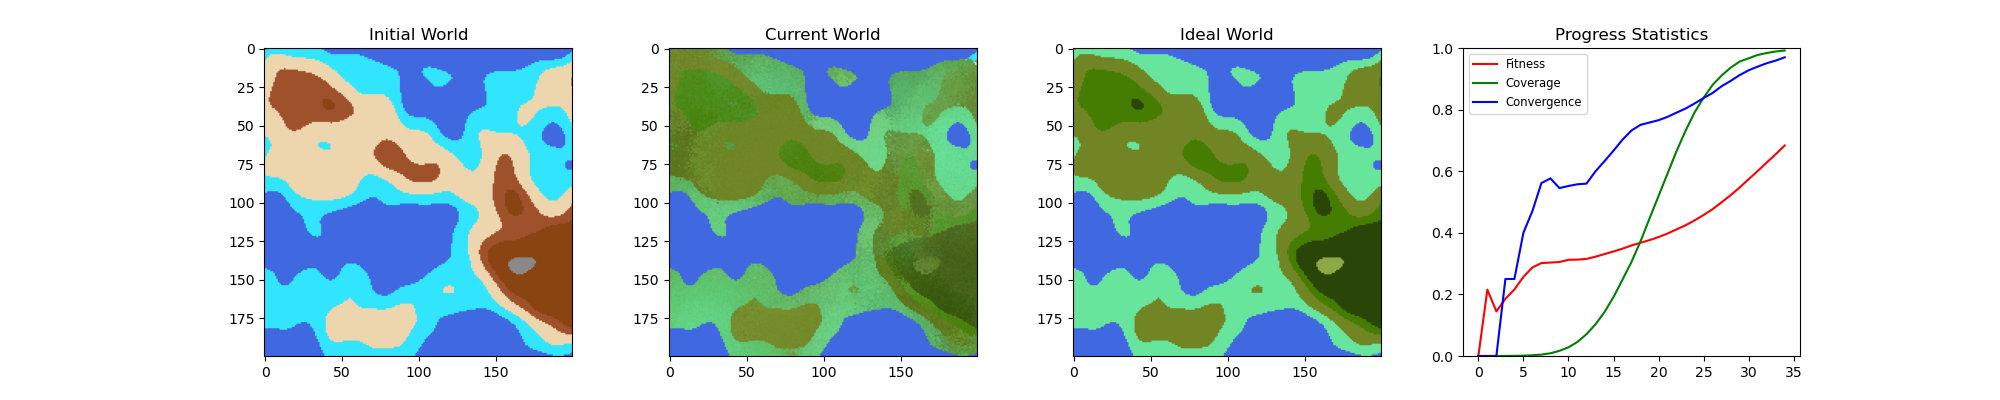
\includegraphics[width=\linewidth]{outputs/q4_frame35.png}
        
        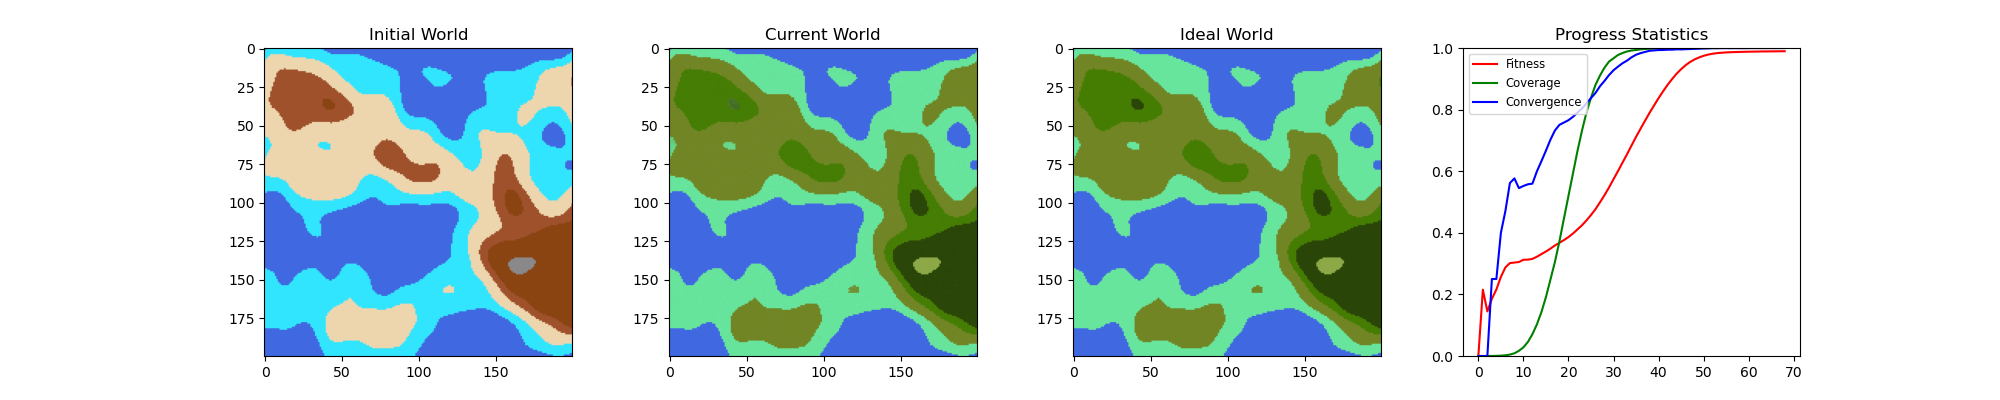
\includegraphics[width=\linewidth]{outputs/q4_frame69.png}
        \end{center}

        \item \textbf{Text responses}

        \begin{enumerate}[(i)]
            \item \textbf{Question 4a}. When life initially starts to spread across the map, the fitness curve is extremely volatile, but eventually it smooths out. Why is this?

            \begin{solution}
                
            \end{solution}

            \item \textbf{Question 4b}. You might notice that the Coverage progression curve tends to match a sigmoid curve. Give a conjecture as to why this might be.

            \begin{solution}
                
            \end{solution}
        \end{enumerate}
    \end{enumerate}
    \end{problem}
    \clearpage
    
\end{problems}

\includepdf[pages=-]{outputs/pocket_planet.pdf}

\end{document}
